\pgfmathsetseed{123456789}%
\tikzset{expressed/.style={-stealth,shorten <=4pt,shorten >=6pt,ultra thick}}%
\tikzset{potential/.style={-stealth,shorten <=4pt,shorten >=6pt,very thick,dotted}}%
\usetikzlibrary{calc}

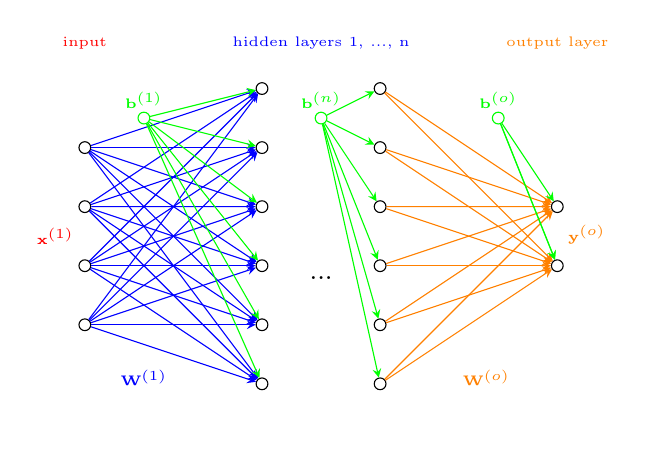
\begin{tikzpicture}[scale=1.5] 
\foreach \i in {0,...,3} \node[draw,circle,inner sep=1.5pt] (input\i) at (0,\the\numexpr0.5*\i+.5+0.75) {};
\foreach \i in {0,...,5} \node[draw,circle,inner sep=1.5pt] (hidden\i) at (1.5,\the\numexpr0.5*\i+0.75) {};
\foreach \i in {0,...,5} \node[draw,circle,inner sep=1.5pt] (hiddenl\i) at (2.5,\the\numexpr0.5*\i+0.75) {};
\foreach \i in {0,...,1} \node[draw,circle,inner sep=1.5pt] (output\i) at (4,\the\numexpr0.5*\i+1+.75) {};

% connectors input -> hidden
\foreach \i in {0,...,3}
\foreach \j in {0,...,5} \draw[-stealth,blue!100!white] (input\i) -- (hidden\j);

% connectors hidden -> output
\foreach \i in {0,...,5}
\foreach \j in {0,...,1} \draw[-stealth,orange!100!white] (hiddenl\i) -- (output\j);

% labels
\draw (input3) ++ (0.0,0.25+.5) node[red,above] {\tiny input};
\draw (output1) ++ (0.0,0.25+1.) node[orange,above] {\tiny output layer};
\draw (hidden5) ++ (0.5,0.25) node[blue,above] {\tiny hidden layers 1, ..., n};

%\draw (input0) ++ (-0.25,-0.20) node[red!100!white,above] {\tiny $x_1$};
\draw (input1) ++ (-0.25,.10) node[red!100!white,above] {\tiny $\mathbf{x}^{(1)}$};

%\draw (input1) ++ (-0.25,-0.20) node[red!100!white,above] {\tiny $x_0$};
%\draw (hiddenl5) ++ (0.0,0.25) node[blue,above] {\tiny hidden (n)};
\draw (output0) ++ (0.25,.10) node[orange,above] {\tiny $\mathbf{y}^{(o)}$};	
\draw (output0) ++ (0.25-2.25,-0.20) node[black,above] {...};	

% bias nodes
\node[color=green,draw,circle,inner sep=1.5pt] (bias1) at (0.5,5*0.5+0.5) {};
\draw (bias1) ++ (0.0,0.0) node[green,above] {\tiny $\textbf{b}^{\text{(1)}}$};

\node[color=green,draw,circle,inner sep=1.5pt] (bias3) at (0.5+1.5,5*0.5+0.5) {};
\draw (bias3) ++ (0.0,0.0) node[green,above] {\tiny $\textbf{b}^{\text{(n)}}$};

\node[color=green,draw,circle,inner sep=1.5pt] (bias2) at (2.25+1.25,5*0.5+0.5) {};
\draw (bias2) ++ (0.0,0.0) node[green,above] {\tiny $\textbf{b}^{\text{(o)}}$};

% bias connectors
\foreach \i in {0,...,5} \draw[-stealth,green!100!white] (bias1) -- (hidden\i);
\foreach \i in {0,...,5} \draw[-stealth,green!100!white] (bias3) -- (hiddenl\i);
\foreach \i in {0,...,1} \draw[-stealth,green!100!white] (bias2) -- (output\i);
\draw[-stealth,green!100!white] (bias2) -- (output0);

% weight labels
\draw (input0) ++ (0.5,-.6) node[blue!100!white,above] {\tiny $\textbf{W}^{\text{(1)}}$};
\draw (hiddenl0) ++ (.9,-0.1) node[orange!100!white,above] {\tiny $\textbf{W}^{\text{(o)}}$};

\node[draw,color=white] (dummy) at (0,0.5) {};
\end{tikzpicture}